
\chapter{遗忘理论在反应式系统中的应用}
\label{chapter04}
%{\em 本章针对第\ref{chapter01}章提出的问题(2)探讨使用遗忘的方法来解决计算反应式系统WSC(SNC)和知识更新。首先给出SNC(WSC)的定义,然后证明任意公式的SNC(WSC)可以规约到命题下的SNC(WSC)。并证明SNC和WSC是一对对偶概念,因此探讨其中一个就足以表示另一个的性质。其次,从遗忘的角度给出了计算SNC(WSC)的方法。基于此,当给定的反应式系统模型为有限状态时,可以事先将该模型用其特征公式表示出来,然后使用遗忘来计算其SNC(WSC)。
%	最后,提出使用遗忘定义
%	%反应式系统中$\CTL$和$\mu$-演算。。。。。。
%	知识更新的方法。

{\em
遗忘可以用于从本体中抽取摘要、隐蔽敏感信息、计算逻辑差等;
WSC和SNC在智能规划和形式化验证里有重要作用,例:在2003年,Lin使用WSC和SNC计算规划问题中的后继状态公理。
%在第\ref{chapter02}章中详细介绍了命题逻辑和模态逻辑S5下使用遗忘计算WSC(SNC)的方法和算法。
本章针对第\ref{chapter01}章提出的问题(2),研究$\CTL$和$\mu$-演算中如何使用遗忘计算反应式系统的SNC(WSC),及使用遗忘定义知识更新。即:
\begin{itemize}
	\item 对于给定的公式$\varphi$、原子命题$q$和原子命题集$V\subseteq \Var(\varphi)$,若满足$q \in \Var(\varphi)-V$,则$q$在$\varphi$和$V$上的SNC等价于公式$\varphi \wedge q$遗忘不在$V$中的原子命题后得到结果;WSC做为SNC的一个对偶概念,有相似的结论。而不终止的系统(包括反应是系统)在本章看作是一个有限的初始结构,任意有限的初始结构(${\cal K}$)都能用其特征公式%(${\cal F}_{\Ha}({\cal K})$)
	来表示(\textbf{给定有限初始结构,如何计算其特征公式将在第\ref{chapter05}章中的介绍,本章只需认为其是一个$\CTL$公式}),因而可以使用遗忘的方法来计算其SNC(WSC)。
	\item 基于遗忘的知识更新通过极小改变现有知识的模型来使其适应新信息,这可以看作是基于模型的更新,且使用这种方法的更新满足katsuno等人提出的八条基本准则\cite{katsuno91mendelzon}。
\end{itemize}


本章其余部分组织如下:首先,第\ref{chapter04:sec:snc}节给出最强必要条件和最弱充分条件的定义,探索这两个概念的相关性质,并给出基于遗忘的计算方法;其次,第\ref{chapter04:sec:update}节提出基于遗忘的知识更新方法,并证明其与基于偏序关系的方法等价;最后,总结本章的研究工作。}

\section{最弱充分条件}
\label{chapter04:sec:snc}
这部分介绍如何使用遗忘理论计算最强必要条件和最弱充分条件。
直观地说,最强必要条件指最一般的结果(the most general consequence),最弱充分条件指最特殊的诱因(the most specific abduction)。
下面给出其形式化定义,本章所说的公式指$\CTL$公式,且这章所有的定义和结论都可以平凡地移到$\mu$-句子下。
\begin{definition}[充分和必要条件]\label{def:NC:SC}
	给定两个公式$\varphi$和$\psi$,$V \subseteq \Var(\varphi)$,$q\in\Var(\varphi)- V$
	和$\Var(\psi)\subseteq V$。
	\begin{itemize}
		\item 若$\varphi \models q \rto \psi$,则称$\psi$是$q$在$V$和$\varphi$上的{\em 必要条件(necessary condition,NC)};
		\item 若$\varphi \models \psi\rto q$,则称$\psi$是$q$在$V$和$\varphi$上的{\em 充分条件(sufficient condition,SC)};
		\item 若$\psi$是$q$在$V$和$\varphi$上的必要条件,且对于任意$q$在$V$和$\varphi$上的必要条件$\psi'$,都有$\varphi\models\psi\rto\psi'$,则称$\psi$是$q$在$V$和$\varphi$上的{\em 最强必要条件(strongest necessary condition,SNC)};
		\item 若$\psi$是$q$在$V$和$\varphi$上的充分条件,且对于任意$q$在$V$和$\varphi$上的充分条件$\psi'$,都有$\varphi\models\psi'\rto\psi$,则称$\psi$是$q$在$V$和$\varphi$上的{\em 最弱充分条件(weakest sufficient condition,WSC)};
	\end{itemize}
\end{definition}

从上述定义可以看出,SNC(WSC)是$q$在$V$和$\varphi$上的NC(SC)中最强(最弱)的一个。此外,如果公式$\psi$和$\psi'$都是$q$在$V$和$\varphi$上的SNC(WSC),则$\psi \equiv \psi'$。
下面的命题表明SNC和WSC是一对对偶概念。

\begin{proposition}[对偶性]\label{dual}
	令$V$、$q$、$\varphi$和$\psi$为定义\ref{def:NC:SC}出现的符号。
	则$\psi$是$q$在$V$和$\varphi$上的SNC(WSC)当且仅当$\neg \psi$是$\neg q$在$V$和$\varphi$上的WSC(SNC)。
\end{proposition}
\begin{proof}
	(i) 假定$\psi$是$q$在$V$和$\varphi$上的SNC,$\psi'$是$\neg q$在$V$和$\varphi$上SC。
	
	$\varphi \models q \rto \psi$ \\
	$\Rto$ $\varphi \models \neg \psi \rto \neg q$。
	
	这表明$\neg \psi$是$\neg q$在$V$和$\varphi$的SC。
	%Suppose $\psi'$ is any other SC of $\neg q$, and
	%We now show $\varphi \models \psi' \rto \neg \psi$.
	
	$\varphi \models \psi' \rto \neg q$\\
	$\Rto$ $\varphi \models q \rto \neg \psi'$,即:$\neg \psi'$是$q$在$V$和$\varphi$上的NC\\
	$\Rto$ $\varphi \models \psi \rto \neg \psi'$ \hfill (假设)\\
	$\Rto$ $\varphi \models \psi' \rto \neg \psi$。
	
	另一个方向可以类似地证明。
	%      (i) Suppose $\psi$ is the SNC of $q$. Then $\varphi \models q \rto \psi$, and then $\varphi \models \neg \psi \rto \neg q$, i.e., $\neg \psi$ is an
	% SC of $\neg q$. Suppose $\psi'$ is any other SC of $\neg q$: $\varphi \models \psi' \rto \neg q$. Then $\varphi \models q \rto \neg \psi'$, i.e., $\neg \psi'$ is an NC of $q$ on $V$ under $\varphi$.
	% Therefore, $\varphi \models \psi \rto \neg \psi'$ by assumption, and then $\varphi \models \psi' \rto \neg \psi$. This proves that $\neg \psi$ is the WSC of $\neg q$.
	% The proof of the other part of the proposition is similar.
	
	(ii) 可以类似SNC的情形证明。
\end{proof}


在定义\ref{def:NC:SC}中,用公式$\alpha$替换$q$,$V\subseteq \Var(\alpha) \cup \Var(\phi)$,则为公式的最强必要条件和最弱充分条件的定义。
下面的命题表明了原子命题的充分(必要)条件与公式的充分(必要)条件之间的关系:通过计算原子命题的充分(必要)条件来计算公式的充分(必要)条件。



\begin{proposition}\label{formulaNS_to_p}
	给定公式$\Gamma$和$\alpha$, $V \subseteq \Var(\alpha) \cup \Var(\Gamma)$,$q$是不出现在$\Gamma$和$\alpha$中的原子命题。
	$\varphi$是集合$V$上的公式,则$\varphi$是$\alpha$在$V$和$\Gamma$上的SNC(WSC) 当且仅当$\varphi$是$q$在$V$和$\Gamma'$上的SNC(WSC),其中$\Gamma' = \Gamma \cup \{q \lrto \alpha\}$。
\end{proposition}
\begin{proof}
	这里证明SNC的情形,WSC的情形可以类似地证明。
	记$\emph{SNC}(\varphi,\beta,V,\Gamma)$为$\varphi$是$\beta$ 在 $V$和$\Gamma$上的SNC,$\emph{NC}(\varphi,\beta,V,\Gamma)$为$\varphi$是$\beta$在$V$和 $\Gamma$上的NC。
	
	($\Rto$) 下证$\emph{SNC}(\varphi,\alpha,V,\Gamma)\Rto \emph{SNC}(\varphi,q,V,\Gamma')$。假设$\varphi'$是$q$在$V$和$\Gamma'$上的NC。
	
	$\Gamma \models \alpha \rto \varphi$ \hfill  (已知)\\
	$\Rto$ $\Gamma \wedge (q \lrto \alpha) \models \alpha \rto \varphi$\\
	$\Rto$ $\Gamma' \models q \rto \varphi$  \hfill ($q \equiv \alpha$)
	
	$\Gamma' \models q \rto \varphi'$ \hfill (假设) \\
	$\Rto$ $\Gamma' \models \alpha \rto \varphi'$ \hfill ($q \equiv \alpha$)\\
	$\Rto$ $\Muforget(\Gamma', \{q\}) \models \alpha \rto \varphi'$ \hfill ($\IR(\alpha \rto \varphi', \{q\})$, $(\PP)$)\\
	$\Rto$ $\Gamma \models \alpha \rto \varphi'$ \hfill  (引理~\ref{lem:KF:eq})\\
	$\Rto$ $\Gamma \models \varphi \rto \varphi'$ \hfill  (已知: $\emph{SNC}(\varphi,\alpha,V,\Gamma)$)\\
	$\Rto$ $\Gamma' \models \varphi \rto \varphi'$.
	
	总之,$\varphi$是$q$在$V$和$\Gamma'$上的NC,且对任意$q$在$V$和$\Gamma'$上的NC$\varphi'$,有$\Gamma' \models \varphi \rto \varphi'$。因此, $\emph{SNC}(\varphi,q,V,\Gamma')$。
	
	($\Lto$) 下证$\emph{SNC}(\varphi,q,V,\Gamma')\Rto \emph{SNC}(\varphi,\alpha,V,\Gamma)$。假定$\varphi'$是$\alpha$在$V$和$\Gamma$上的NC。
	
	$\Gamma' \models q \rto \varphi$ \hfill  (已知)\\
	$\Rto$  $\Gamma' \models \alpha \rto \varphi$ \hfill  ($q \equiv \alpha$)\\
	$\Rto$  $\Muforget(\Gamma', \{q\}) \models \alpha \rto \varphi$ \hfill ($\IR(\alpha \rto \varphi, \{q\})$, $(\PP)$)\\
	$\Rto$ $\Gamma \models \alpha \rto \varphi$ \hfill  (引理~\ref{lem:KF:eq})
	
	$\Gamma \models \alpha \rto \varphi'$ \hfill  (假设)\\
	$\Rto$ $\Gamma' \models \alpha \rto \varphi'$ \\
	$\Rto$ $\Gamma' \models q \rto \varphi'$ \hfill  ($q \equiv \alpha$)\\
	$\Rto$ $\Gamma' \models \varphi \rto \varphi'$ \hfill (已知:$\emph{SNC}(\varphi,q,V,\Gamma')$)\\
	$\Rto$ $\Muforget(\Gamma', \{q\}) \models \varphi \rto \varphi'$ \hfill ($\IR(\varphi \rto \varphi', \{q\})$, $(\PP)$)\\
	$\Rto$ $\Gamma \models \varphi \rto \varphi'$ \hfill (引理~\ref{lem:KF:eq})
	
	总之,$\varphi$是$\alpha$在$V$和$\Gamma$上的NC,且对任意$\alpha$在$V$和$\Gamma$上的NC$\varphi'$,有$\Gamma \models \varphi \rto \varphi'$。因此, $\emph{SNC}(\varphi,\alpha,V,\Gamma)$。
\end{proof}


%为了对给定原子命题集合下公式的最弱充分条件有个直观的认识,下面给出一个简单的例子。
%下面的例子给出了关于给定原子命题集合下的公式的最弱充分条件的具体体现。

\begin{example}[例\ref{exam:vB}的延续]\label{examp:WSC}
	本例来源于图\ref{exam:vB}中的初始结构${\cal K}_2$。令$\psi = \EXIST \NEXT(s \wedge (\EXIST \NEXT se \vee \EXIST \NEXT \neg d))$、$\varphi = \EXIST \NEXT(s \wedge \EXIST \NEXT \neg d)$、$\Ha =\{d, s, se\}$和$V = \{s, d\}$。下面证明$\varphi$是$\psi$在$V$和${\cal K}_2$上的WSC:
	\begin{itemize}
		\item[(i)] 由已知有$\varphi \models \psi$和$\Var(\varphi) \subseteq V$。此外,$(\Hm, s_0) \models \varphi \wedge \psi$,因此${\cal K}_2 \models \varphi \rto \psi$,即:$\varphi$是$\psi$在$V$和${\cal K}_2$上的SC;
		\item[(ii)] 下证“对任意$\psi$在$V$和${\cal K}_2$上的SC $\varphi'$都有${\cal K}_2 \models \varphi' \rto \varphi$”。易知若${\cal K}_2 \not \models \varphi'$,则${\cal K}_2\models \varphi' \rto \varphi$。
		假设${\cal K}_2 \models \varphi'$。由$\varphi'$是$\psi$在$V$和${\cal K}_2$上的SC可知$\varphi' \models \EXIST \NEXT(s \wedge \phi)$,其中$\phi$是使得$\phi\models \EXIST \NEXT se \vee \EXIST \NEXT \neg d$成立的公式。又$\IR(\varphi', \overline V)$,所以$\phi \models \EXIST \NEXT \neg d$。因此,$\varphi' \models \varphi$且${\cal K}_2 \models \varphi' \rto \varphi$。
	\end{itemize}
\end{example}


如何使用遗忘计算SNC(WSC)是本章讨论的关键问题。下面首先给出其理论基础,然后再做直观的解释。


\begin{theorem}\label{thm:SNC:WSC:forget}
	给定公式$\varphi$、原子命题集$V\subseteq\Var(\varphi)$和原子命题$q\in\Var(\varphi)- V$。
	\begin{itemize}
		\item[(i)] $\CTLforget (\varphi \land q$, $(\Var(\varphi) \cup \{q\}) - V)$是$q$在$V$和$\varphi$上的SNC;
		\item[(ii)]  $\neg\CTLforget (\varphi \land \neg q$, $(\Var(\varphi) \cup \{q\}) - V)$是$q$在$V$和$\varphi$上的WSC。
	\end{itemize}
\end{theorem}
\begin{proof}
	(i) 令${\cal F}=\CTLforget(\varphi \wedge q, (\Var(\varphi) \cup \{q\})- V)$。
	
	
	“NC”部分:由遗忘的定义可知$\varphi \wedge q \models {\cal F}$。因此,$\varphi\models q \rto {\cal F}$,即:${\cal F}$是$q$在$V$和$\varphi$ 上的NC。
	
	“SNC”部分:假设$\psi'$为$q$在$V$和$\varphi$上的任意NC,即:$\varphi\models q \rto \psi'$。由定理\ref{thm:V-bisimulation:EQ} 和 $\emph{IR}(\psi', (\Var(\varphi) \cup \{q\})- V)$可知,若$\varphi \wedge q \models \psi'$,则${\cal F} \models \psi'$。
	由假设可知$\varphi\models q \rto \psi'$,所以$\varphi \wedge {\cal F} \models \psi'$,因此$\varphi \models {\cal F} \rto \psi'$。
	
	由上面两部分可知,${\cal F}$是$q$在$V$和$\varphi$上的SNC。
	
	(ii) 令${\cal F}=\neg \CTLforget(\varphi \wedge \neg q, (\Var(\varphi) \cup \{q\})- V)$。
	由命题\ref{dual}可知,对任意命题$q'$,$\CTLforget$ $(\varphi \wedge q', (\Var(\varphi) \cup \{q'\})- V)$是$q'$在$V$和$\varphi$上的SNC,当且仅当
	$\neg \CTLforget(\varphi \wedge q', (\Var(\varphi) \cup \{q'\})- V)$是$\neg q'$在$V$和$\varphi$上的WSC。
	由(i)可知$\CTLforget(\varphi \wedge q', (\Var(\varphi) \cup \{q'\})- V)$是$q'$在$V$和$\varphi$上的SNC,所以$\neg \CTLforget(\varphi \wedge q', (\Var(\varphi) \cup \{q'\})- V)$是$\neg q'$在$V$和$\varphi$上的WSC。令$q=\neg q'$,可得${\cal F}$是 $q$在 $V$ 和 $\varphi$上的WSC。
\end{proof}

令${\cal F}=\CTLforget(\varphi \wedge q, (\Var(\varphi) \cup \{q\})- V)$。上面的定理可以直观地解释如下:由遗忘理论的定义可知$\varphi \wedge q \models {\cal F}$,这说明
${\cal F}$是 $q$在 $V$和$\varphi$上的NC;对任意与$(\Var(\varphi) \cup \{q\})- V$无关的公式$\psi$,若$\varphi \wedge q \models \psi$,则由表达性定理可知${\cal F} \models \psi$。

值得注意的是,定理~\ref{thm:SNC:WSC:forget}中,当考虑的公式为$\mu$-公式时,要求出现在$\varphi$中的变元都包含在$V$中。

由第\ref{chapter05}章可知,任意有限的初始结构都能由一个$\CTL$公式表示,所以由上面的定理自然地就能得到给定有限初始结构下的SNC和WSC。
\begin{corollary}\label{thm:inK:SNC}
	令${\cal K}= (\Hm, s_0)$为初始结构,其中$\Hm=(S,R,L,s_0)$为有限原子命题集$\Ha$上的初始-Kripke结构,$V \subseteq \Ha$且$q\in V' = \Ha - V$。则:
	\begin{itemize}
		\item[(i)] $\CTLforget({\cal F}_{\Ha}({\cal K}) \wedge q, V')$是$q'$在$V$和${\cal K}$上的SNC;
		\item[(ii)] $\neg \CTLforget({\cal F}_{\Ha}({\cal K}) \wedge \neg q, V')$是$q'$在$V$和${\cal K}$上的WSC。
	\end{itemize}
\end{corollary}

\begin{example}[例~\ref{car_manufacturing}的延续]
	\label{exam:SNCandWSC}
令$\Ha=\{d,se,sp,s\}$和$V=\{d,se\}$,求$s$在$V$和初始结构${\cal K} = (\Hm,s_0)$ 上的WSC,其中$\Hm$为例~\ref{car_manufacturing}中初始状态为$s_0$的汽车制造企业模型结构。

由定理~\ref{thm:inK:SNC}可知,$s$在$V$和初始结构${\cal K} = (\Hm,s_0)$上的WSC为$\neg \CTLforget({\cal F}_{\Ha}({\cal K}) \wedge \neg s, \{s\}$ $\cup \{sp\})$。

由于涉及到后文中遗忘的计算方法,本例的详细计算过程放到第~\ref{chapter05:sec:model}。
%\begin{align*}
%&	\CTLforget({\cal F}_{\Ha}({\cal K}) \wedge \neg s, \{s\} \cup \{sp\})\\
%&	\equiv \CTLforget(\CTLforget({\cal F}_{\Ha}({\cal K}) \wedge \neg s, \{sp\}), \{s\})\\
%&	\equiv \CTLforget(\CTLforget({\cal F}_{\Ha}({\cal K}), \{sp\})\wedge \neg s, \{s\}).
%\end{align*}
%
%${\cal K}_1 \models \CTLforget({\cal F}_{\Ha}({\cal K}), \{sp\})$\\
%$\LRto$ 存在${\cal K}_1' \lrto_{\{sp\}} {\cal K}_1$使得${\cal K}_1' \models {\cal F}_{\Ha}({\cal K})$和\\
%$\LRto$ 存在${\cal K}_1' \lrto_{\{sp\}} {\cal K}_1$使得${\cal K}_1' \lrto_{\emptyset} {\cal K}$\\
%$\LRto$ 存在${\cal K}_1' \lrto_{\{sp\}} {\cal K}$和${\cal K}_1' \models {\cal F}_{V\cup \{s\}}({\cal K})$ \hfill (定理~\ref{CF})\\
%$\LRto$ ${\cal K}_1 \models {\cal F}_{V\cup \{s\}}({\cal K})$。
%
%由此可知,$ \CTLforget({\cal F}_{\Ha}({\cal K}), \{sp\}) \equiv {\cal F}_{V\cup \{s\}}({\cal K})$。所以要计算$\neg \CTLforget({\cal F}_{\Ha}({\cal K}) \wedge \neg s, \{s\} \cup \{sp\})$,只需计算$\neg \CTLforget({\cal F}_{V\cup \{s\}}({\cal K})\wedge \neg s, \{s\})$。令$V' = V \cup \{s\} = \{d,se,s\}$,则$\overline{V'} = \{sp\}$。
%
%
%容易检查除了$s_2$和$s_4$是$\overline{V'}$-互模拟的,其余都是$V'$-可区分的,且$\dis_{V'}(\Hm, s_i, s_j, 0)$,其中$i\not =j$且$i$和$j$不能同时分别取值2和4。
%因此可以计算$\Hm$关于$V'$的特征数为:
%$$ch(\Hm, V')=\max\{k\mid s,s'\in S \text{ 且 } \dis_{V'}({\cal M},s,s',k)\} = 0\hbox{。}$$
%
%
%所以,可以由以下步骤计算${\cal K}_2$关于$V$的特征公式:
%\begin{align*}
%	{\cal F}_{V'}(\Tr_0(s_0)) &= d \wedge \neg se \wedge \neg s, \qquad \qquad \qquad \qquad \quad {\cal F}_{V'}(\Tr_0(s_1)) = \neg d \wedge \neg se \wedge s, \\
%	{\cal F}_{V'} (\Tr_0(s_2)) &= {\cal F}_{V'} (\Tr_0(s_4)) = \neg d \wedge se \wedge \neg s,  \qquad  {\cal F}_{V'}(\Tr_0(s_3) = \neg d \wedge \neg se\wedge \neg s,\\
%	{\cal F}_{V'}(\Hm, s_0)& \equiv d \wedge \neg se \wedge \neg s \wedge \\
%	& \ALL \GLOBAL(d \wedge \neg se \wedge \neg s \rto \ALL\NEXT(\neg d \wedge \neg se \wedge s))\wedge \\
%	& \ALL \GLOBAL(\neg d \wedge \neg se \wedge s \rto [\ALL\NEXT((\neg d \wedge se \wedge \neg s) \vee (\neg d \wedge \neg se\wedge \neg s)) \wedge\\ &\EXIST\NEXT(\neg d \wedge se \wedge \neg s) \wedge \EXIST\NEXT (\neg d \wedge \neg se\wedge \neg s)]) \wedge\\
%	& \ALL \GLOBAL(\neg d \wedge \neg se\wedge \neg s \rto \ALL\NEXT(d \wedge \neg se \wedge \neg s)) \wedge\\
%	& \ALL \GLOBAL(\neg d \wedge se \wedge \neg s \rto \ALL\NEXT(d \wedge \neg se \wedge \neg s)).
%\end{align*}
%令:
%\begin{align*}
%\varphi_1&  = d \wedge \neg se \wedge \neg s \rto \ALL\NEXT(\neg d \wedge \neg se \wedge s)\equiv \neg d \vee se \vee s \vee \ALL\NEXT(\neg d \wedge \neg se \wedge s),\\
%\varphi_2& = \neg d \wedge \neg se \wedge s \rto \ALL\NEXT(\neg d \wedge se \wedge \neg s) \equiv d \vee  se \vee \neg s \vee\\
%& [\ALL\NEXT((\neg d \wedge se \wedge \neg s) \vee (\neg d \wedge \neg se\wedge \neg s)) \wedge\EXIST\NEXT(\neg d \wedge se \wedge \neg s) \wedge \EXIST\NEXT (\neg d \wedge \neg se\wedge \neg s)],\\
%\varphi_3 &=\neg d \wedge \neg se\wedge \neg s \rto \ALL\NEXT(d \wedge \neg se \wedge \neg s)\equiv d \vee se \vee s \vee \ALL\NEXT(d \wedge \neg se \wedge \neg s),\\
%\varphi_4 &= \neg d \wedge se \wedge \neg s \rto \ALL\NEXT(d \wedge \neg se \wedge \neg s)\equiv d \vee \neg se \vee s \vee \ALL\NEXT(d \wedge \neg se \wedge \neg s).
%\end{align*}
%此外,令
%\begin{align*}
%	& \psi_1 = \neg d \vee se \vee s && \psi_2 = d \vee  se \vee \neg s \\
%	& \psi_3 = d \vee se \vee s && \psi_4 = d \vee \neg se \vee s\\
%	& \alpha_1 = \ALL\NEXT(\neg d \wedge \neg se \wedge s) && \alpha_2 = \ALL\NEXT((\neg d \wedge se \wedge \neg s) \vee (\neg d \wedge \neg se\wedge \neg s))\\
%	& \alpha_3 = \EXIST\NEXT(\neg d \wedge se \wedge \neg s) \wedge \EXIST\NEXT (\neg d \wedge \neg se\wedge \neg s) && \alpha_4 = \ALL\NEXT(d \wedge \neg se \wedge \neg s)\\
%	& \alpha_5 = \ALL\NEXT(d \wedge \neg se \wedge \neg s) && \psi = d \wedge \neg se \wedge \neg s.
%\end{align*}
%则,
%\begin{align*}
%	& \psi \wedge \varphi_1 \wedge \varphi_2 \wedge \varphi_3\wedge \varphi_4 
%	\equiv (\psi \wedge \psi_1 \wedge \psi_2 \wedge \psi_3 \wedge \psi_4) \vee (\psi \wedge \psi_1 \wedge \psi_2 \wedge \psi_3 \wedge \alpha_5) \vee\\
%	& (\psi \wedge \psi_1 \wedge \psi_2 \wedge \alpha_4 \wedge \psi_4) \vee (\psi \wedge \psi_1 \wedge \psi_2 \wedge \alpha_4 \wedge \alpha_5) \vee\\
%	& (\psi \wedge \psi_1 \wedge \alpha_2 \wedge \alpha_3 \wedge \psi_3 \wedge \psi_4) \vee (\psi \wedge \psi_1 \wedge \alpha_2 \wedge \alpha_3 \wedge \psi_3 \wedge \alpha_4) \vee \\
%	& (\psi \wedge \psi_1 \wedge \alpha_2 \wedge \alpha_3 \wedge \alpha_4 \wedge \psi_4) \vee (\psi \wedge \psi_1 \wedge \alpha_2 \wedge \alpha_3 \wedge \alpha_4 \wedge \alpha_5) \vee\\
%	& (\psi \wedge \alpha_1 \wedge \psi_2 \wedge \psi_3 \wedge \psi_4) \vee (\psi \wedge \alpha_1 \wedge \psi_2 \wedge \psi_3 \wedge \alpha_5)\vee\\
%	& (\psi \wedge \alpha_1 \wedge \psi_2 \wedge \alpha_4 \wedge \psi_4) \vee (\psi \wedge \alpha_1 \wedge \psi_2 \wedge \alpha_4 \wedge\alpha_5)\vee \\
%	& (\psi \wedge \alpha_1 \wedge \alpha_2 \wedge \alpha_3 \wedge \psi_3 \wedge \psi_4) \vee (\psi \wedge \alpha_1 \wedge \alpha_2 \wedge \alpha_3\wedge \psi_3 \wedge \alpha_5) \vee \\
%	& (\psi \wedge \alpha_1 \wedge \alpha_2 \wedge \alpha_3 \wedge \alpha_4 \wedge \psi_4) \vee (\psi \wedge \alpha_1 \wedge \alpha_2 \wedge \alpha_3 \wedge \alpha_4 \wedge \alpha_5).\\
%	\\
%%\end{align*}
%%\begin{align*}
%	& \varphi_1 \wedge \varphi_2 \wedge \varphi_3\wedge \varphi_4 
%	 \equiv (\psi_1 \wedge \psi_2 \wedge \psi_3 \wedge \psi_4) \vee (\psi_1 \wedge \psi_2 \wedge \psi_3 \wedge \alpha_5) \vee\\
%	& (\psi_1 \wedge \psi_2 \wedge \alpha_4 \wedge \psi_4) \vee (\psi_1 \wedge \psi_2 \wedge \alpha_4 \wedge \alpha_5) \vee\\
%	& (\psi_1 \wedge \alpha_2 \wedge \alpha_3 \wedge \psi_3 \wedge \psi_4) \vee ( \psi_1 \wedge \alpha_2 \wedge \alpha_3 \wedge \psi_3 \wedge \alpha_4) \vee \\
%	& ( \psi_1 \wedge \alpha_2 \wedge \alpha_3 \wedge \alpha_4 \wedge \psi_4) \vee ( \psi_1 \wedge \alpha_2 \wedge \alpha_3 \wedge \alpha_4 \wedge \alpha_5) \vee\\
%	& (\alpha_1 \wedge \psi_2 \wedge \psi_3 \wedge \psi_4) \vee ( \alpha_1 \wedge \psi_2 \wedge \psi_3 \wedge \alpha_5)\vee\\
%	& (\alpha_1 \wedge \psi_2 \wedge \alpha_4 \wedge \psi_4) \vee ( \alpha_1 \wedge \psi_2 \wedge \alpha_4 \wedge\alpha_5)\vee \\
%	& (\alpha_1 \wedge \alpha_2 \wedge \alpha_3 \wedge \psi_3 \wedge \psi_4) \vee (\alpha_1 \wedge \alpha_2 \wedge \alpha_3\wedge \psi_3 \wedge \alpha_5) \vee \\
%	& ( \alpha_1 \wedge \alpha_2 \wedge \alpha_3 \wedge \alpha_4 \wedge \psi_4) \vee ( \alpha_1 \wedge \alpha_2 \wedge \alpha_3 \wedge \alpha_4 \wedge \alpha_5).
%\end{align*}
%所以,
%\begin{align*}
%	&\neg \CTLforget({\cal F}_{V\cup \{s\}}({\cal K})\wedge \neg s, \{s\}) \\
%	& \equiv \neg \CTLforget({\cal F}_{V\cup \{s\}}({\cal K}), \{s\})\\
%	& \equiv \neg \CTLforget(\psi \wedge \ALL \GLOBAL(\varphi_1 \wedge \varphi_2 \wedge \varphi_3\wedge \varphi_4),\{s\})\\	
%	& \equiv \neg(\CTLforget(\psi \wedge \varphi_1 \wedge \varphi_2 \wedge \varphi_3\wedge \varphi_4, \{s\}) \wedge \ALL \GLOBAL \CTLforget(\varphi_1 \wedge \varphi_2 \wedge \varphi_3\wedge \varphi_4, \{s\}))\\
%	& \equiv  \neg \bigg(\Big(d \vee \big((d\vee se) \wedge \ALL\NEXT(d \wedge \neg se)\big) \vee \big((d \vee se \vee \ALL\NEXT \neg d) \wedge \EXIST\NEXT(\neg d \wedge se) \wedge \EXIST\NEXT(\neg d \wedge \neg se)\big) \\
%	& \vee (d \wedge \ALL\NEXT(\neg d \wedge \neg se)) \vee \big((d\vee \neg se) \wedge \EXIST\NEXT\neg d\big) \Big) \wedge\\
%	& \ALL \GLOBAL\Big(\big((d \vee se) \wedge \ALL\NEXT(d \wedge \neg se)\big) \vee \big(\ALL\NEXT \neg d \wedge \EXIST\NEXT(\neg d \wedge se) \wedge\\
%	& \EXIST\NEXT(\neg d \wedge \neg se)\big) \vee \big((d\vee se) \wedge \ALL\NEXT(\neg d \wedge \neg se)\big) \vee \EXIST\NEXT \neg d\Big)
%	\bigg)\hbox{。}
%\end{align*}
\end{example}


\section{知识更新}\label{chapter04:sec:update}
本小节介绍遗忘的另一个应用:知识更新(Knowledge update)。
具体说来,本节将使用遗忘定义知识更新,使得用这种方式定义的知识更新满足下面由Katsuno和Mende- lzon提出的基本条件\cite{katsuno91mendelzon}:
\begin{itemize}
	\item (U1)  $\Gamma \diamond \varphi \models \varphi$;
	\item (U2) 若$\Gamma \models \varphi$,则$\Gamma \diamond \varphi \equiv \Gamma$;
	\item (U3) 若$\Gamma$和$\varphi$都是可满足的,则$\Gamma \diamond \varphi$是可满足的;
	\item (U4) 若$\Gamma_1\equiv \Gamma_2$且$\varphi_1 \equiv \varphi_2$,则$\Gamma_1 \diamond \varphi_1 \equiv \Gamma_2 \diamond \varphi_2$;
	\item (U5) $(\Gamma \diamond \varphi) \wedge \psi \models \Gamma \diamond(\varphi \wedge \psi)$;
	\item (U6) 若$\Gamma \diamond \varphi \models \psi$且$\Gamma \diamond \psi \models \varphi$,则$\Gamma \diamond \varphi \equiv \Gamma \diamond \psi$;
	\item (U7) 若$\Gamma$有唯一一个模型,则$(\Gamma \diamond \varphi) \wedge (\Gamma \diamond \psi) \models \Gamma \diamond (\varphi \vee \psi)$;
	\item (U8) $(\Gamma_1 \vee \Gamma_2) \diamond \varphi \equiv (\Gamma_1 \diamond \varphi) \vee  (\Gamma_2 \diamond \varphi)$。
\end{itemize}
其中,$\diamond$为知识更新操作,$\varphi \diamond \psi$表示用$\psi$更新$\varphi$得到的结果。

本小节假设所有初始结构都是有限的,即:状态来源于有限状态空间且$\Ha$为有限原子命题集。

%下面定理显然成立:
%\begin{theorem}\label{thm:initModel}
%	给定公式$\varphi$和原子命题集$V \subseteq \cal A$。存在一个公式$\psi$使得:
%	\[
%	(\Hm,s_0) \models \psi \mbox{ 当且仅当存在 } (\Hm',s_0')\in\Mod(\varphi) \mbox{ 使得 } (\Hm,s_0) \lrto_V (\Hm',s_0') % \mbox{ and } \Hm' \models \phi.
%	\]
%	其中$(\Hm,s_0)$和$(\Hm',s_0')$都是有限的初始结构。
%\end{theorem}
%\begin{proof}
%	令$\psi=\Muforget(\varphi, V)$(或$\psi=\CTLforget(\varphi, V)$)。由遗忘的定义可知,对任意的${\cal K} \models \psi$存在一个${\cal K}' \models \varphi$使得${\cal K} \lrto_V {\cal K}'$,且对每一个${\cal K}' \in \Mod(\varphi)$都有${\cal K}' \models \psi$。
%	此时,容易证明对任意的有限初始结构${\cal K}$,若${\cal K} \models \psi$,则存在一个${\cal K}'$使得${\cal K}' \models \varphi$且${\cal K} \lrto_V {\cal K}'$。
%	
%	此外,对任意的${\cal K}' \in \Mod(\varphi)$,由(\W)可知存在${\cal K}' \models \psi$。又${\cal K} \lrto_V {\cal K}'$,所以$\Hm \models \psi$。
%\end{proof}


%定理\ref{thm:initModel}表明模型结构被限制到有限初始结构下的$\mu$-演算下遗忘理论也是封闭的。
由第\ref{chapter05}章可知,任意$\Ha$上的有限初始结构$\Hm$(为了简化符号,本节用初始Kripke结构$\Hm$代替初始结构$(\Hm,s_0)$)都能用一个$\CTL$公式——特征公式${\cal F}_{\Ha}(\Hm)$来表示。%,此公式也是$\mu$-句子。
给定公式$\varphi$和$\psi$,$V_{min}\subseteq \Ha$为使得$\CTLforget(\varphi, V_{min}) \wedge \psi$可满足的极小子集。
%,记$\varphi = \CTLforget({\cal F}_{\Ha}({\cal K}), V_{min})$,其中$V_{min} \subseteq \Ha$是使得$\varphi$可满足的极小子集。
此外,记
$$\bigcup_{V_{min}\subseteq \Ha} \Mod(\CTLforget({\cal F}_{\Ha}(\Hm), V_{min}) \wedge \psi)$$ 
%$$\bigcup_{V_{min}\subseteq \Ha} \Mod(\CTLforget({\cal F}_{\Ha}({\cal K}), V_{min}))$$
为所有$\CTLforget({\cal F}_{\Ha}(\Hm), V_{min}) \wedge \psi$的模型集合的并集。
此时,可如下定义$\mu$-演算下的知识更新操作:


\begin{definition}\label{def:KU}
	给定公式$\Gamma$和$\varphi$。知识更新操作$\diamond_{\CTL}$定义如下:
	\[
	\Mod(\Gamma \diamond_{\CTL} \varphi) = \bigcup_{\Hm \in \Mod(\Gamma)} \bigcup_{V_{min}\subseteq \Ha} \Mod(\CTLforget({\cal F}_{\Ha}(\Hm), V_{min}) \wedge \varphi),
	\]
	其中,${\cal F}_{\Ha}(\Hm)$是$\Hm$在$\Ha$上的特征公式,$V_{min} \subseteq \Ha$是使得$\CTLforget({\cal F}_{\Ha}(\Hm), V_{min})$可满足的极小子集。
\end{definition}

直观上,$\Gamma \diamond_{\CTL} \varphi$表示:通过极小化改变$\Gamma$的模型,使其与$\varphi$的模型一致来更新$\Gamma$。
%换句话说,定义\ref{def:KU}通过极小化改变$\Gamma$的每个模型,使得该模型能够满足$\varphi$来更新原有的知识$\Gamma$。
所以,这样定义的知识更新是一种基于模型的知识更新方法。

此外,$\CTL$知识更新也可以用类似于命题逻辑里基于偏序关系的更新来定义:令$I$,$J_1$和$J_2$为三个解释,即:原子命题集;则$J_1$比$J_2$更接近$I$(记为:$J_1 \leq_{I,pma} J_2$)当且仅当$\Diff(I, J_1) \subseteq \Diff(I, J_2)$,其中$\Diff(X, Y) =\{p\in \Ha \mid X(p) \not = Y(p)\}$。那么命题逻辑知识更新——用$\psi$更新$\Gamma$,即为$\psi$的关于偏序关系$\leq_{I,pma}$的所有极小模型的集合($I$是$\Gamma$的模型),即:
$$\Mod(\Gamma \diamond_{pma} \psi) = \bigcup_{I \in \Mod(\Gamma)} Min(\Mod(\psi), \leq_{I,pma}).$$
其中,$Min(\Mod(\psi), \leq_{I,pma})$是$\psi$的关于偏序关系$\leq_{I,pma}$的极小模型集。

类似地,这里定理有限初始结构之间关于另一个初始结构的偏序关系。
\begin{definition}\label{def:closer}
	给定三个有限初始结构$\Hm$、$\Hm_1$和$\Hm_2$,$\Hm_1$比$\Hm_2$更接近$\Hm$(记为$\Hm_1 \leq_{\Hm} \Hm_2$),当且仅当对任意$V_2 \subseteq \Atom$,若$\Hm_2 \lrto_{V_2} \Hm$,则存在$V_1 \subseteq V_2$使得$\Hm_1 \lrto_{V_1} \Hm$。
	$\Hm_1 <_{\Hm} \Hm_2$当且仅当$\Hm_1 \leq_{\Hm} \Hm_2$且$\Hm_2 \not \leq_{\Hm} \Hm_1$。
\end{definition}
%\begin{definition}\label{def:closer}
%	给定三个有限初始结构${\cal K}$、${\cal K}_1$和${\cal K}_2$,${\cal K}_1$比${\cal K}_2$更接近${\cal K}$(记为${\cal K}_1 \leq_{{\cal K}} {\cal K}_2$)当且仅当对任意使得${\cal K}_2 \lrto_{V_2} {\cal K}$成立的$V_2 \subseteq \Atom$都存在一个$V_1 \subseteq V_2$使得${\cal K}_1 \lrto_{V_1} {\cal K}$。
%	 ${\cal K}_1 <_{{\cal K}} {\cal K}_2$当且仅当${\cal K}_1 \leq_{{\cal K}} {\cal K}_2$且${\cal K}_2 \not \leq_{{\cal K}} {\cal K}_1$。
%\end{definition}

在这种情形下,若$\Hm_1 \leq_{\Hm} \Hm_2$,则存在一个原子命题的极小集$V_{min}$使得$\Hm_1 \lrto_{V_{min}} \Hm$,且对任意$V\subseteq \Ha$,若$\Hm_2 \lrto_V \Hm$则$V_{min}\subseteq V$且$\Hm_1 \lrto_V \Hm$。
\begin{example}
	\textcolor{red}{令$\Hm= (S, R, L, r)$、$\Hm_1 = (S_1, R_1, L_1, r_1)$、$\Hm_2 = (S_2, R_2, L_2, r_2)$为三个初始结构(如图~\ref{fig:partialo}),其中$S = S_1 = S_2 = \{s_0, s_1\}$,$r=r_1=r_2= s_0$,$R=R_1=R_2=\{(s_0, s_1), (s_1, s_1)\}$,$L(s_0) = \{ch, j\}$,$L_1(s_0) = L_2(s_0) = \{ch\}$,$L(s_1) = L_1(s_1)=\emptyset$,$L_2(s_1) = \{j\}$。}
	
	可以检查$\Hm \lrto_{\{j\}} \Hm_1$,$\Hm \lrto_{\{j,ch\}} \Hm_2$,$\{j\}\subseteq \{j,ch\}$,且对任意原子命题集$V' \subset \{j\}$(或$V' \subset \{j,ch\}$),有$\Hm \not\lrto_{V'} \Hm_1$(或$\Hm \not \lrto_{V'} \Hm_2$)。
	因此,$\Hm_1 \leq_{\Hm} \Hm_2$。
	\begin{figure}[h]%
		\centering
		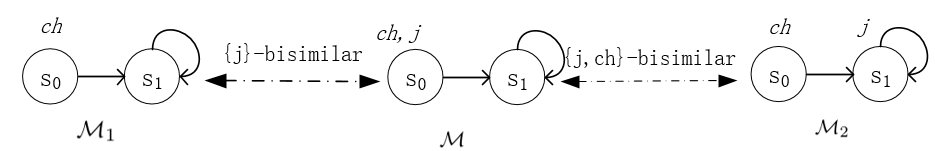
\includegraphics[width=12cm,height=2cm]{figures/chapter06/partial_order.png}
		\caption{初始结构间的$\leq_{\Hm}$关系。}\label{fig:partialo}
		
		% $s_0$ is labeled by $\{ch, j\}$, $t_0$ is labeled by $\{j\}$, and $s_1$, $s_2$, and $t_1$ are labeled by $\emptyset$.}\label{fig:bisim}
	\end{figure}
\end{example}

给定有限初始结构集$M$和有限初始结构$\Hm$,用$Min(M,$ $\leq_{\Hm})$表示$M$中关于偏序关系$\leq_{\Hm}$的极小有限初始结构集。则$\leq_{\Hm}$与知识更新操作$\diamond_{\CTL}$有如下关系。

\begin{theorem}\label{thm:minU}
	给定$\mu$-句子$\Gamma$和$\varphi$,则:
	\[\Mod(\Gamma \diamond_{\CTL} \varphi) = \bigcup_{\Hm\in \Mod(\Gamma)} Min(\Mod(\varphi), \leq_{\Hm}).
	\]
\end{theorem}
\begin{proof}
	$\Hm'\in \Mod(\Gamma \diamond_{\CTL} \varphi)$\\
	$\LRto$ 存在$\Hm \models \Gamma$和极小子集$V_{min} \subseteq \Ha$,使得$\Hm' \in \Mod(\Muforget({\cal F}_{\Ha}(\Hm)$, $V_{min}) \wedge \varphi)$\\
	$\LRto$ 存在$\Hm \models \Gamma$和$V_{min}\subseteq \Ha$,使得$\Hm \lrto_{V_{min}} \Hm'$和$\Hm' \models \varphi$,且$V_{min}$是使得$\Muforget({\cal F}_{\Ha}(\Hm)$, $V_{min}) \wedge \varphi$可满足的$\Ha$极小子集\\
	$\LRto$ 存在$\Hm \models \Gamma$,使得对任意$\Hm''\models \varphi$,$\Hm' \leq_{\Hm} \Hm''$\\
	$\LRto$ $\Hm' \in Min(\Mod(\varphi), \leq_{\Hm})$。
\end{proof}


从定理\ref{thm:minU}可以看出,通过遗忘定义的知识更新操作与通过有限初始结构间的偏序关系定义的知识更新一致,且通过遗忘定义的知识更新操作满足Katsuno和Mendelzon提出的八条基本条件。

\begin{theorem}\label{thm:U1toU8}
	知识更新操作$\diamond_{\CTL}$满足Katsuno和Mendelzon提出的基本条件(U1)-(U8)。
\end{theorem}
\begin{proof}
	(U1). 由定理~\ref{thm:minU}可知,$\Mod(\Gamma \diamond_{\mu} \varphi) \subseteq \Mod(\varphi)$,因此$\Gamma \diamond_{\mu} \varphi \models \varphi$。
	
	(U2). $\Hm'\in \Mod(\Gamma \diamond_{\mu} \varphi)$\\
	$\LRto$ 存在$\Hm \models \Gamma$,使得对任意$\Hm'' \models \varphi$ 和$V \subseteq \Ha$,$\Hm'' \lrto_{V} \Hm$ 蕴涵$\Hm' \lrto_{V} \Hm$\\
	$\LRto$ 存在$\Hm \models \Gamma$和$V_{min} = \emptyset$,使得$\Hm' \lrto_{V_{min}} \Hm$ \hfill ($\Gamma \models \varphi$)\\
	$\LRto$ $\Hm'\models \Gamma$。
	
	
	容易证明$\diamond_{\mu}$满足(U3)和(U4)。
	%We now prove (U5).
	
	(U5). $\Hm'\models (\Gamma \diamond_{\mu} \varphi) \wedge \psi$\\
	$\Rto$  存在$\Hm \models \Gamma$,使得对任意$\Hm'' \models \varphi \wedge \psi$ 和$V \subseteq \Ha$,$\Hm'' \lrto_{V} \Hm$蕴涵$\Hm' \lrto_{V} \Hm$\\
	$\Rto$ 存在$\Hm \models \Gamma$和$V_{min} \subseteq \Ha$,使得$\Hm' \lrto_{V_{min}} \Hm$和$\Hm' \models \varphi \wedge \psi$,其中$V_{min}$是使得$\Hm' \lrto_{V_{min}} \Hm$的$\Ha$的极小子集\\
	% 且对任意的$\Hm''\models \psi$ 若$\Hm''\lrto_V \Hm$则$\Hm' \lrto_{V} \Hm$且$V_{min} \subseteq V$ \\
	$\Rto$ $\Hm' \models \Gamma \diamond_{\mu} (\varphi \wedge \psi)$。
	
	
	
	(U6). $\Hm'\models \Gamma \diamond_{\CTL} \varphi$\\
	$\LRto$ 存在$\Hm \models \Gamma$,使得对任意$\Hm'' \models \varphi$ 和$V \subseteq \Ha$,$\Hm'' \lrto_{V} \Hm$ 蕴涵$\Hm' \lrto_{V} \Hm$\\
	$\LRto$ 存在$\Hm \models \Gamma$和$V_{min} \subseteq \Ha$,使得$\Hm' \lrto_{V_{min}} \Hm$,其中$V_{min}$是使得$\Muforget({\cal F}_{\Ha}(\Hm_1), V_{min}) \wedge \varphi$ 和 $\Muforget({\cal F}_{\Ha}(\Hm_1), V_{min}) \wedge \psi$是一致的 \hfill ($\Gamma \diamond_{\CTL} \varphi \models \psi$, $\Gamma \diamond_{\CTL} \psi \models \varphi$) \\ % \qquad \qquad \textcolor[RGB]{0,134,139}{$\%$({\em Otherwise, suppose that $V\subset V_{min}$ s.t. $\Muforget({\cal F}_{\Ha}(\Hm_1), V) \wedge \psi$ is consistent as well. Then, $\Muforget({\cal F}_{\Ha}(\Hm_1), V)$ $\wedge \varphi$ should also be consistent by $\Gamma \diamond_{\CTL} \varphi \models \psi$, which contradicts to the fact that $V_{min}$ is the minimal set of atoms s.t. $\Muforget({\cal F}_{\Ha}(\Hm_1), V_{min}) \wedge \varphi$ is consistent.})} \\
	$\LRto$ 存在$\Hm \models \Gamma$,使得对任意$\Hm'' \models \psi$ 和$V \subseteq \Ha$,$\Hm'' \lrto_{V} \Hm$ 蕴涵$\Hm' \lrto_{V} \Hm$\\
	$\LRto$ $\Hm' \models \Gamma \diamond_{\CTL} \psi$。
	
	
	
	(U7). $\Hm' \models (\Gamma \diamond_{\CTL} \varphi) \wedge (\Gamma \diamond_{\CTL} \psi)$,且设$\Hm$是$\Gamma$的唯一模型\\
	$\Rto$ 存在两个极小子集$V_1, V_2 \subseteq \Ha$,使得$\Hm \lrto_{V_1} \Hm'$ 和$\Hm \lrto_{V_2} \Hm'$\\
	$\Rto$ 存在两个极小子集$V_1, V_2 \subseteq \Ha$,使得$\Hm' \models \Muforget({\cal F}_{\Ha}(\Hm), V_1) \wedge \varphi$ 和 $\Hm' \models \Muforget({\cal F}_{\Ha}(\Hm),$ $V_2) \wedge \psi$是一致的\\
	%$\Rto$ $\Hm' \lrto_{V_1 \cap V_2} \Hm$\\
	$\Rto$ $\Hm' \models \Muforget({\cal F}_{\Ha}(\Hm), V_1 \cap V_2)$,$\Hm' \lrto_{V_1 \cap V_2} \Hm$,$V_1 = V_2$\\
	$\Rto$  $V_1$是使得$\Muforget({\cal F}_{\Ha}(\Hm), V_1) \wedge (\varphi \vee \psi)$可满足的极小子集\\ %\qquad  \textcolor[RGB]{0,134,139}{$\%$({\em Otherwise, suppose that $V_3\subset V_1$ s.t. $\Muforget({\cal F}_{\Ha}(\Hm),$ $V_3) \wedge (\varphi \vee \psi)$ is satisfiable. Then $\Muforget({\cal F}_{\Ha}(\Hm),$ $V_3) \wedge \varphi$ or $\Muforget({\cal F}_{\Ha}(\Hm),$ $V_3) \wedge \psi$ is satisfiable. Without loss of generality, suppose that $\Muforget({\cal F}_{\Ha}(\Hm), V_3) \wedge \varphi$ is satisfiable, $V_1$ is not the minimal set, a contradiction.})}\\
	$\Rto$ $\Hm' \models \Gamma \diamond_{\CTL} (\varphi \vee \psi)$。
	
	
	
	(U8). $\Hm \models (\Gamma_1 \vee \Gamma_2) \diamond_{\CTL} \varphi$ \\
	$\LRto$ 存在$\Hm_1 \models \Gamma_1$ (或$\Hm_1 \models \Gamma_2$) 和一个极小子集$V_{min}$,使得$\Hm \lrto_{V_{min}} \Hm_1$\\
	$\LRto$ $\Hm \models (\Gamma_1 \diamond_{\CTL} \varphi) \vee (\Gamma_2 \diamond_{\CTL} \varphi)$。
\end{proof}


\begin{example}
	令$\Ha=\{ch, j\}$、$\varphi = \nu X. j \wedge ch \wedge \EXIST \NEXT \EXIST \NEXT X$、 $\psi= \nu X. \neg j \wedge ch \wedge \EXIST \NEXT \EXIST \NEXT X$且Kripke结构的状态空间为 $\{s_0,s_1\}$,则用$\psi$更新$\varphi$计算如下:
	\begin{align*}
		\Mod(\varphi) = & \{((1), r=s_0, L(s_0)=\{ch,j\}, L(s_1)=\{ch,j\}), \\
		& ((2),  r=s_1, L(s_1)=\{ch,j\}, L(s_0)=\{ch,j\}),\\
		& ((3),  r=s_0, L(s_0)=\{ch,j\}, L(s_1)={\cal C}), \\
		& ((4),  r=s_1, L(s_1)=\{ch,j\}, L(s_0)={\cal C}), \\
		& ((5),  r=s_0, L(s_0)=\{ch,j\}, L(s_1)={\cal C}), \\
		& ((6),  r=s_1, L(s_1)=\{ch,j\}, L(s_0)={\cal C}), \dots\}\\
		\Mod(\psi) = & \{((1), r=s_0, L(s_0)=\{ch\}, L(s_1)=\{ch\}),\\
		& ((2), r=s_1, L(s_1)=\{ch\}, L(s_0)=\{ch\}),\\
		& ((3), r=s_0, L(s_0)=\{ch\}, L(s_1)={\cal C}),\\
		& ((4), r=s_1, L(s_1)=\{ch\}, L(s_0)={\cal C}), \\
		& ((5), r=s_0, L(s_0)=\{ch\}, L(s_1)={\cal C}),\\
		& ((6), r=s_1, L(s_1)=\{ch\}, L(s_0)={\cal C}), \dots\}
	\end{align*}
	其中,四元组$((i), r= s_k, L(s_0)=V_1, L(s_1)=V_1)$表示Kripke结构$(S,r,R,L)$,其中$S=\{s_0, s_1\}$、$r=s_k$ ($r\in \{0,1\}$)、转换关系如图~\ref{fig:knoup}中的(i) ($i \in \{1,2,3,4,5,6\}$\footnote{这里只列出部分转换关系,其余转换关系可以容易地枚举出来。})、$s_0$ 和$s_1$分别被 $V_1 \subseteq \{ch,j\}$ 和 $V_2\subseteq \{ch,j\}$标记且${\cal C} \in \{\emptyset, \{j\}, \{ch\}, \{j,ch\}\}$。
	
	$\Mod(\varphi \diamond_{\mu} \psi) = \bigcup_{\Hm\in \Mod(\varphi)} Min(\Mod(\psi), \leq_{\Hm})$,根据定义~\ref{def:closer}容易检查$\Mod(\varphi \diamond_{\mu} \psi) = \Mod(\psi)$。直观地说,由于在$\psi$中$j$在偶数状态不再为真、$ch$保持为真且$\psi$和$\varphi$都不知道模型偶数状态的信息,因而用$\psi$更新$\varphi$得到的结果为 $\psi$自身。
	\begin{figure}[h]%
		\centering
		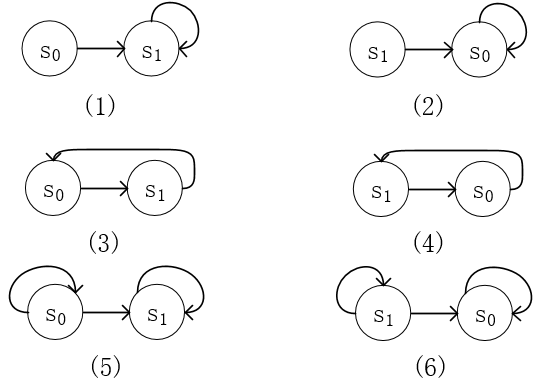
\includegraphics[width=8cm]{knowledge_update.png}
		\caption{状态空间为$\{s_0,s_1\}$的六个Kripke结构示意图}\label{fig:knoup}
		
		% $s_0$ is labeled by $\{ch, j\}$, $t_0$ is labeled by $\{j\}$, and $s_1$, $s_2$, and $t_1$ are labeled by $\emptyset$.}\label{fig:bisim}
	\end{figure}
\end{example}


\section{本章小结}\label{sec:chapter04-conclusion}

本章讨论了如何使用遗忘计算最强必要条件(最弱充分条件)和定义知识更新。特别地,本章首先给出了SNC(WSC)的定义,表明SNC和WSC是一对对偶概念,因而只要知道其一就能知道另一个。其次,结论表明任意公式的SNC(WSC)可以转换成原子命题的SNC(WSC)来计算,并给出使用遗忘计算原子命题在给定条件下的SNC(WSC)的方法。
最后,分别给出使用遗忘和偏序关系的方法定义知识更新,并证明了这两种定义等价且满足Katsuno等人提出的八条准则。

